\documentclass [12pt] {article}
\makeatletter
\setlength{\@fptop}{0pt}
\makeatother
\usepackage{graphicx}
\usepackage{color}
\usepackage{listings}
\lstset{ %
language=C++,                % choose the language of the code
basicstyle=\footnotesize,       % the size of the fonts that are used for the code
numbers=left,                   % where to put the line-numbers
numberstyle=\footnotesize,      % the size of the fonts that are used for the line-numbers
stepnumber=1,                   % the step between two line-numbers. If it is 1 each line will be numbered
numbersep=5pt,                  % how far the line-numbers are from the code
backgroundcolor=\color{white},  % choose the background color. You must add \usepackage{color}
showspaces=false,               % show spaces adding particular underscores
showstringspaces=false,         % underline spaces within strings
showtabs=false,                 % show tabs within strings adding particular underscores
frame=single,           % adds a frame around the code
tabsize=2,          % sets default tabsize to 2 spaces
captionpos=b,           % sets the caption-position to bottom
breaklines=true,        % sets automatic line breaking
breakatwhitespace=false,    % sets if automatic breaks should only happen at whitespace
escapeinside={\%*}{*)}          % if you want to add a comment within your code
}

\title{\vspace{-2cm}Assignment \#3: Predator-Prey Model}
\author{Timmy Nguyen}
\begin{document}
\maketitle
\section{A Brief Introduction}
In this lab, I am observing the relationship between the prey and the predator and to create a model illustrating the results from the relationship. The prey model is represented by the equation, $V_{t+1} = V_t + rV - aV_tP_t$. Whie the predator model is represented by the model, $P_{t+1} = P_t + abV_tP_t - dP_t$.

\section{Results}

\subsubsection{Prey and Predator Population Size Over Time}
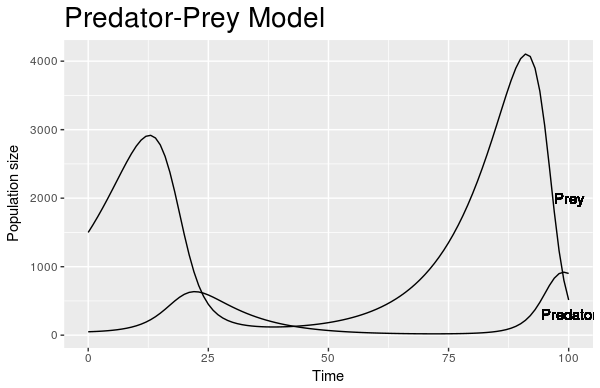
\includegraphics[scale=0.9]{Rplot.png} \\
% 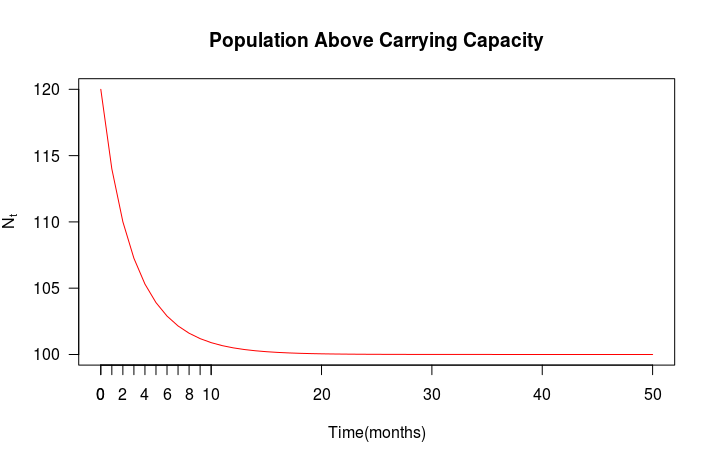
\includegraphics[scale=0.6]{graph2.png}
\newpage

\subsection{Predator vs. Prey Population Size}
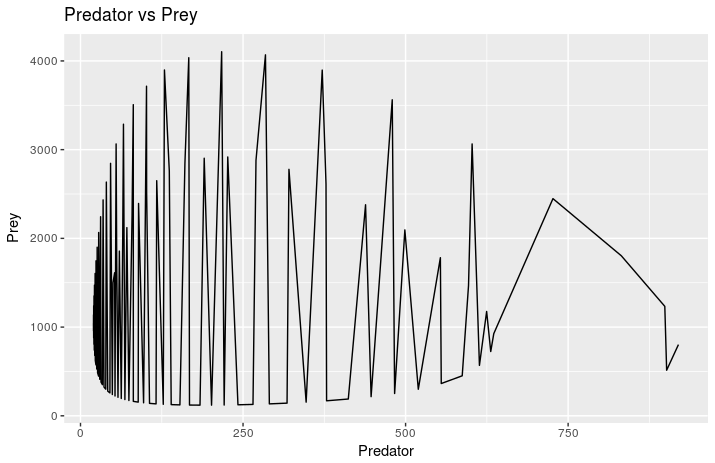
\includegraphics[scale=0.9]{Rplot02.png}

\section{Conclusion}
By analyzing the results from the graph, I concluded that the rise of the prey population is due to a lower population size of the predator. When the prey population decreases, then the graph shows an increase in the predator's population.
\newpage

\section{Appendix}
\subsubsection{C/C++ Code for Exponential Growth Model}
\lstinputlisting[language=c]{Predator_Prey_model.cpp}
\subsubsection{R Code for Generating Predator and Prey Population Size Over Time}
\lstinputlisting[language=R]{Predator_Prey_Model.R}

\subsection{R code for Generating Predator vs Prey Population Size }
\lstinputlisting[language=R]{Predator_VS_Prey_Graph.R}


\end{document}

